\documentclass[11pt]{article}
\usepackage[margin=.8in]{geometry}
\usepackage{amsmath,amssymb,graphicx,hyperref}
\setlength{\parindent}{0pt}\setlength{\parskip}{6pt}
\begin{document}
\begin{center}{\Large Actual residual pair certificates have quadratic coverage}\\
23 November 2026 --- local unsigned Lean component evidence\end{center}
\textbf{Actual scoped conclusion.}
An explicitly exhibited residual factorization
\[
 \langle h\rangle=I(P)^4J,\qquad h\ne0,\qquad J=I(Q)I(R)
\]
in actual nonsingular rational point ideals derives the actual group relation
\(4P+Q+R=0\). Repeated points are allowed. For a fixed finite base \(B\),
if \(Q,R\in B\) and multiplication by four is injective on the certified target
set \(T\), then \(|T|\le |B|^2\).
If the actual finite group order is coprime to four and \(|B|^2\) is smaller
than that order, an actual target lacks this particular pair certificate
(PCC-20261123-7eef03) [pcc:unverified].
\begin{center}
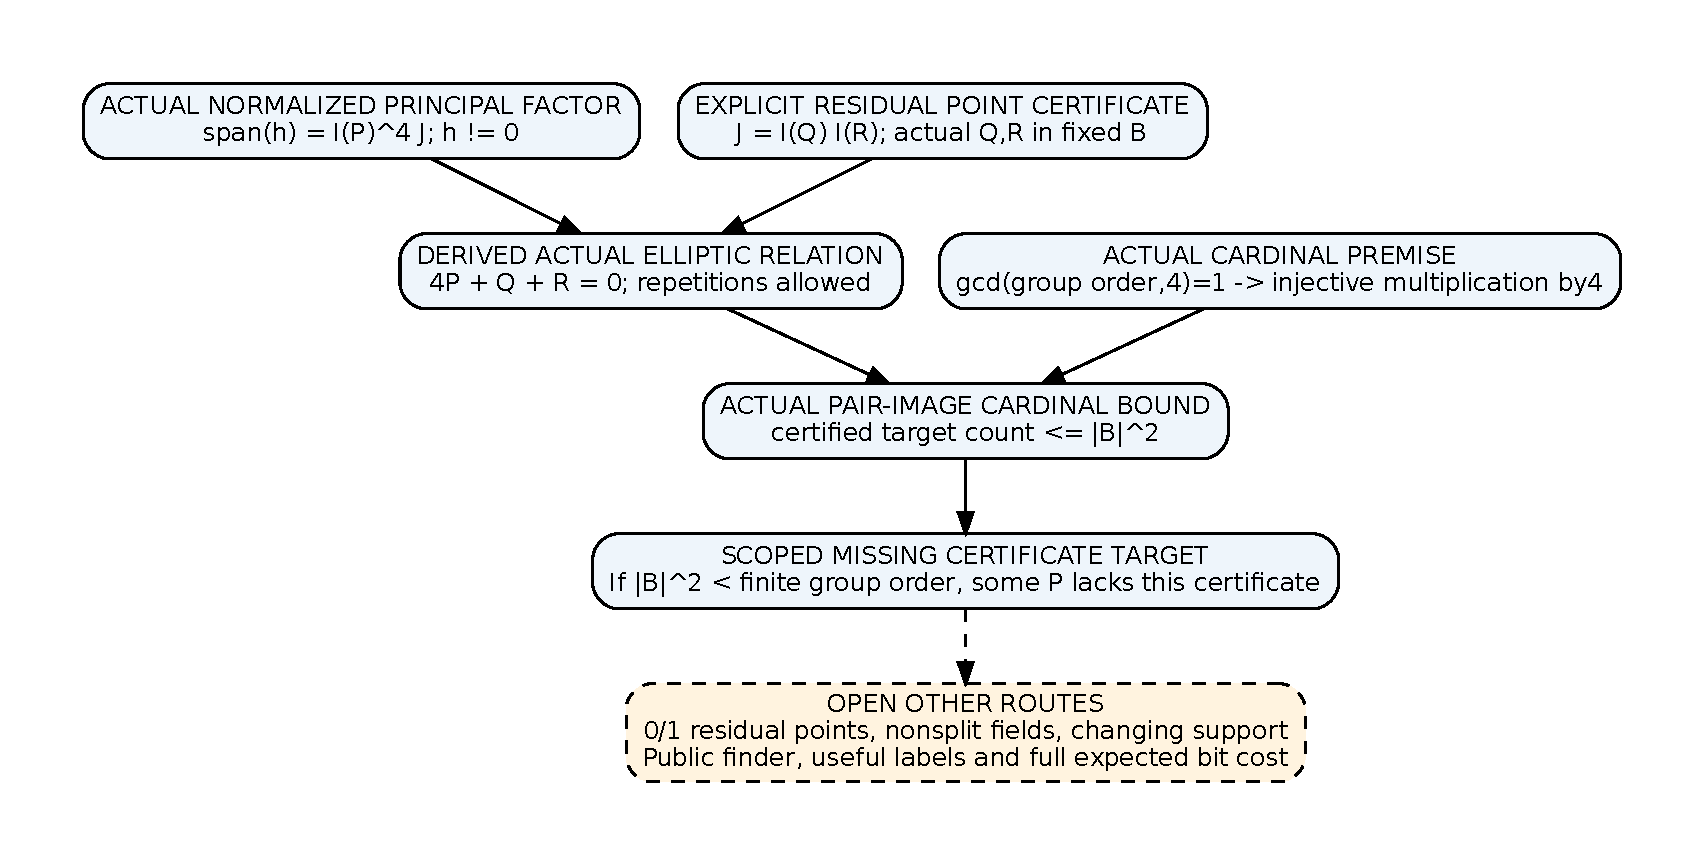
\includegraphics[height=5.25in,width=.96\linewidth,keepaspectratio]{residual-coverage-dependencies-001.pdf}
\end{center}
This is a limitation of the stated fixed two-rational-affine-point certificate
family. It does not cover all residual field cases or give a universal
algorithm lower bound. No factorization finder or scalar labels are supplied
by the small residual quotient dimension.
\newpage
\begin{center}{\Large Actual maps, proof scope and discriminating successor}\end{center}
\textbf{Group transport without a supplied principal point product.}
The exact actual ideal equality and explicit residual point factorization
construct the principal point product on \(\operatorname{Fin}(4)\sqcup\iota\).
The existing actual class-group/elliptic-group theorem then derives
\(4P+\sum_iQ_i=0\), without distinct-coordinate assumptions. The principal
point product is derived, while residual point factorization remains an explicit
certificate condition [pcc:unverified].

\textbf{Actual cardinal argument.}
The map \(P\mapsto4P\) sends certified targets into
\[
 \{-(Q+R): (Q,R)\in B\times B\}.
\]
Existing public finite-set image and product cardinality laws give
\(|T|\le|B|^2\) under the explicit injectivity premise.
Public coprime-cardinality multiplication makes that map bijective when the
actual group cardinal is coprime to four. Taking all actual group points then
exhibits a missing certificate target if \(|B|^2\) is smaller than group order.
This standard cardinal/group algebra is reused, not claimed as a novel attack
or a runtime lower bound [pcc:unverified].

\textbf{Checks and proof map.}
Source077/build083/local040 checks197 local statements, eleven new since186,
exit zero, zero warnings, all printed foundations standard;255 direct input
bindings are checked. PCC-20261123-7eef03 remains unsigned local data outside
historical shared Transport53/57 audit/fresh [pcc:unverified].
\begin{center}\begin{tabular}{l}
\texttt{OrientationActualResidualGroup}\\
\texttt{residual\_point\_product}\\
\texttt{residual\_point\_group\_relation}\\[4pt]
\texttt{OrientationActualResidualCoverage}\\
\texttt{pair\_relation\_targets\_card}\\
\texttt{actual\_pair\_certificate\_targets\_card}\\
\texttt{four\_injective\_of\_coprime\_card}\\
\texttt{exists\_target\_without\_pair\_certificate}
\end{tabular}\end{center}
The actual pair certificate definition records the target, nonzero function,
exact ideal factorization and the two actual rational points in \(B\).

\textbf{Sources and preservation.}
Source \texttt{NormGroupBridge} supplies the existing actual principal-product
to point-sum theorem. Public Mathlib finite-set cardinal laws and
\texttt{OrderOfElement} provide the pair-image count and coprime multiplication
bijection. KB access remained unavailable as previously recorded.
Rejected074 dependent sum,075 unused-variable warning and076 product-opacity /
Boolean-order errors remain exact;077 uses the public product bridge and actual
commutativity. No private-body, linter, class, resource or trust override was used.

\textbf{Next discriminating actions.}
Close the zero- and one-rational-point residual cases with the identity padded
into the fixed base. Keep nonsplit degree-two residue fields explicit.
Then test growing or asymmetric support whose point contribution survives
normalization; paired support currently divides both coefficients and cancels.
Require an actual known-label/finder/coverage and complete bit-cost bridge before
calling a surviving construction a useful index-calculus relation algorithm.
\end{document}
